\vspace{-0.1in}
\section{Introduction}
\vspace{-0.05in}
\label{sec:intro}
Existing datacenters are based on a server-centric architecture, where a small amount of the various resources needed for computing tasks (CPU, memory, storage) are tightly integrated within a single server. While server-centric architectures have been the mainstay for decades, recent efforts suggest a paradigm shift: a {\em disaggregated} datacenter (\dis) that is architected as a pool of decoupled resources, with each resource type built as a standalone resource blade, interconnected via a unified network fabric as shown in Figure~\ref{fig:dc}. In such a datacenter, the aggregation of resources needed by a job is then logical (allocated by a software scheduler) rather than physical (dictated by hardware).

Multiple small-scale prototypes of disaggregated hardware exist already --- Intel RSA~\cite{rsa}, HP ``the machine''~\cite{hptm}, Facebook's disaggregated rack~\cite{fdr}, and SeaMicro~\cite{seamicro}, as well as research prototypes like Firebox~\cite{firebox}, soNUMA~\cite{sonuma}, and disaggregated memory blades~\cite{ddcHwDesign1}.

\begin{figure*}[!t]
\centering 
\subfigure[Current datacenter] {
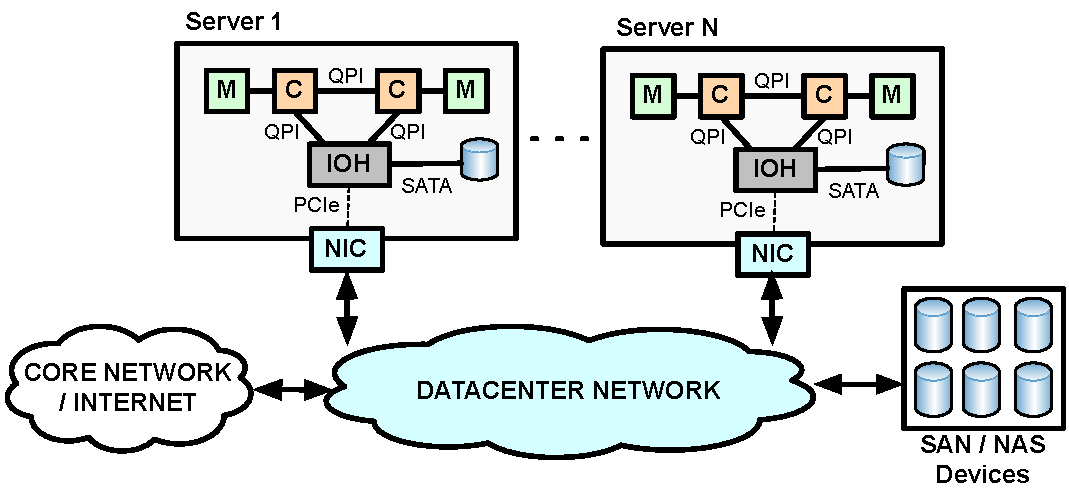
\includegraphics[width=3.05in]{img/DC_before_4.pdf}
\label{fig:dc_before}
}
\hfill
\subfigure[Disaggregated datacenter] {
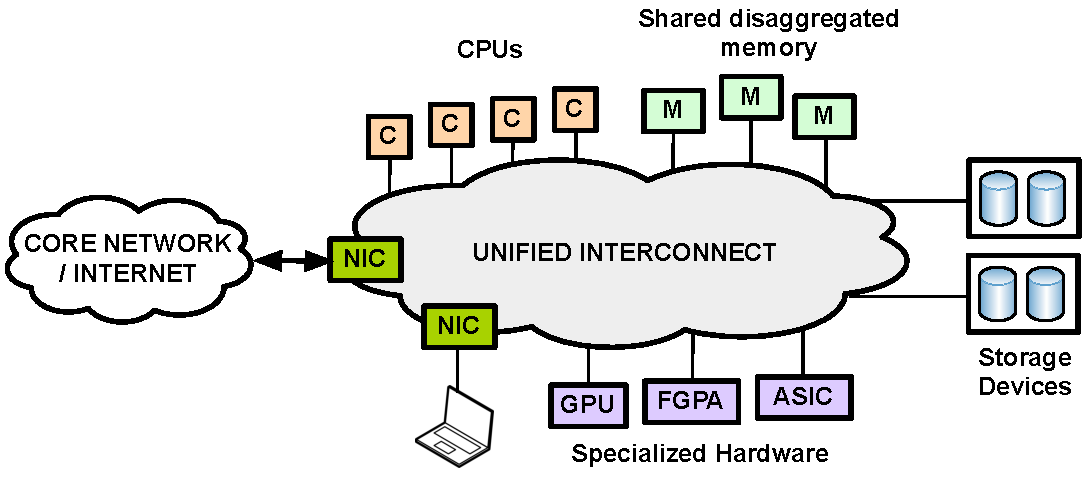
\includegraphics[width=3.05in]{img/DC_after_2.pdf}
\label{fig:dc_after}
}
\tightcaption{Architectural differences between server-centric and resource-centric datacenters}
\label{fig:dc}
\end{figure*}




Resource disaggregation stands to benefit both hardware developers and datacenter operators. %is beneficial along several dimensions. 
For hardware vendors, disaggregation makes computing hardware more modular and hence 
easier to build and evolve. 
An ongoing challenge for hardware architects is that technologies for CPUs, memory, storage, etc. have very different cost, performance, and power scaling trends and this constrains their integration. For example, architects have warned of an impending `memory capacity wall' because of which co-locating compute and memory in a single server will not be sustainable~\cite{ddcHwDesign1}. 
Similarly, as new technologies or specialized computing needs arise~\cite{memristors,nvram,reg-ex-hardware,gpus}, having standalone per-resource blades avoids the burdensome process of redoing the process of integration, motherboard design, and server factor form planning. Disaggregation offers similar benefits to operators, giving them finer-grained control over how they  provision, upgrade, and schedule individual resources.
%Finally, resource disaggregation allows overcoming the technology barriers (imbalance between memory and CPU capacity, power dissipation issues, etc), potentially enabling new technological advances. 

While disaggregation offers the above benefits, it introduces new challenges for the underlying network fabric. The inter-resource communication that used to be contained within a server is now spread across the network fabric. This not only increases the load on the network but makes low latency communication critical. The network will, thus, be one of the key enabling or blocking factors to resource disaggregation. 

Unfortunately, the network support required for resource disaggregation is, at best, poorly understood. The existing deployments of disaggregated datacenters are either small scale or proprietary, with few details available publicly~\cite{rsa, hptm, fdr, seamicro}.

This paper takes a step in building an understanding of the requirements and challenges in enabling network support for \dis. Our approach is workload-driven; we use five common, yet diverse, workloads including batch processing jobs from Hadoop and Spark, point queries from Memcached~\cite{memcached} and ElasticSearch~\cite{elastic} and streaming applications from Storm~\cite{storm}. Using these workloads, we aim to answer three questions through a combination of emulations and simulation: 

\begin{itemize}[leftmargin=*]
	\itemsep0em
		\item What support will be needed from the network, in terms of latency and bandwidth, to maintain the application-level performance within $10\%$ of server-centric architecture? \rc{$\gets$ a lot of people asked yesterday: why $10\%$?}
	\item How will the network traffic change in DDC? What are the important design parameters that impact traffic patterns?
    \item Can existing transport protocols meet the above requirements? 
\end{itemize}

\noindent
To date, there is no consensus on the granularity at which resource disaggregation will happen --- at the rack-scale, pod-scale, or an extreme of datacenter scale. Moreover, as briefly discussed above, resource disaggregation enables flexibility in choice of provisioning and sharing of resources adding to the degrees of freedom in design of \dis architecture. Given that our focus is on understanding the network support for \dis (rather than proposing a \dis architecture), we consider the new degrees of freedom --- scale of disaggregation, CPU-memory disaggregation, data placement and access, etc. --- as design parameters that may impact our study. Our key findings are:

\begin{itemize}[leftmargin=*]
	\itemsep0em
		\item To maintain the application-level performance within $10\%$ of current server-centric architecture, \dis will require a full-bisection bandwidth network with $40$Gbps bandwidth capacity, and an end-to-end latency of $5\mu$s, ignoring the optimizations that disaggregation enables. These requirements highlight the challenge: while $40$Gbps (or even $100$Gbps) is feasible with existing technology, the key to resource disaggregation is to achieve low end-to-end latency between resource blades. \rqc{Independent of the design parameters in DDC;} \rc{$\gets$ removed this sentence; it is not entirely true that this result is independent of design parameters; eg, this result depends on local cache size}
	    \item As expected, DDC traffic volume increases; however, in comparison to existing datacenter traffic studies~\cite{srikanth, theo}, we observe: (a) relatively more homogeneous spatial and temporal distribution of traffic; (b) concentration of traffic within a smaller range of flow sizes; and (c) more homogeneous traffic volume distribution between short flows and long flows. While the design parameters significantly impact DDC traffic characteristics, the high-level observations above suggest that many common tenets that have guided datacenter design to date no longer hold. 
        \item Short memory-bound flows dominating the \dis traffic, combined with a more homogeneous spatial and temporal traffic distribution present favorable characteristics for existing transport protocols~\cite{pfabric} to meet \dis requirements. However, depending on the design parameters, existing protocols may be subjected to new challenges namely, robustness across workloads and application-level policies on flow prioritization (\S\ref{sec:existing}). \rc{$\gets$ requires better arguments} \rqc{room for improvement?}
\end{itemize}

\noindent
Given the relatively forward-looking nature of our study, several caveats apply to our observations. First, our results use workloads from applications designed for server-centric architectures. Our study is not comprehensive in existing workloads; besides, both the applications and the workloads may evolve alongside \dis architectures thus impacting  our results. Second, the focus of our study is on network support for \dis; to that end, we ignore several systems related challenges. It may very well turn out that the latter have a more profound impact on \dis architectures and applications. In this sense, one might view our study as an exploration of whether it is possible to avoid the network from becoming the bottleneck in \dis architectures. Finally, many aspects of the overall \dis context we consider do not exist yet. Consequently, we must make assumptions (\eg, resource blade organization, data layout, etc.). We make what we believe are sensible choices, state these choices explicitly and in many cases, explore the impact of the choices made on our results. However, our results are dependent on these choices and more experience is needed to confirm their validity.

\cut{
\noindent
\sr{Add a list of caveats/disclaimers as follows\ldots}
\begin{itemize} 
\item our results are based on the workloads we study; not comprehensive
\item we focus on net design, ignore many systems questions; may still well turn out that the latter matters more; in this sense one might view our study as seeing whether the network can `get out of the way’ \cite{};
\item because our study is forward looking, many aspects of the overall context we’re considering don’t exist yet so we must make assumptions - e.g., data layout, how resources blades are organized, etc.  We 
\end{itemize} }